\section{Filesystems}

As mentioned before, one of an operating system's tasks is the management of resources.
One of those resources is storage. There are three main reasons why storage (and many other
hardware devices) are handled by the OS.
\begin{enumerate}
\item The OS provides a layer of abstraction for the running application programs. 
\item Talking to the hardware reqires a certain privilege level (IO privileges).
\item Operating systems provide consistency across all files, users and processes.
\end{enumerate}

Remembering file names is easier for humans than remembering the physical location of the file on the storage medium. Filesystems handle
the numbers and metadata of the file and the mapping of file names to actual file contents. It
controls and organizes how data is stored and retrieved from a storage device. It structures a storage
device in files and directories and their metadata. Modern filesystems also provide mechanism for
error detection and encryption.

\subsection{Storage devices}

Storage devices such as hard disks, floppy disks, USB flash drive and SSDs have no notion of files.
These devices only know \textit{sectors}. Sectors are the smallest container a storage device
can work on and they can usually hold 512, 2048 or 4096 bytes of data. These devices are attached to
the computer through I/O (input/output) ports, sometimes in the form of SATA connectors or USB slots, where they can
receive commands from or send information to the CPU on the system. A command can be to \texttt{READ} sector number $x$ to RAM
address $y$ or \texttt{WRITE} from RAM address $y$ to sector $x$. This command is sent through
specific I/O pins from the CPU to the storage device. The device then executes the command or returns
an error if for example sector $x$ is not a valid sector. Remembering which files are located on
which sector numbers is tedious for both humans and computers. This is where filesystems come to help.
\footnote{Storage devices, from: Tech21, \today }

\subsection{The superblock}

The heart of the file system is a datastructure that contains every single file and directory: the
superblock. It holds the \textit{metadata} (i.e. data about data) about every single file/directory,
including its location on the storage device and additional information such as permissions, creation
and modification date but not the contents of the file itself. Said metadata of a file/directory is
grouped together in a structure called \textit{inode}. Every inode is of equal size and is associated
with an inode number. In essence, the superblock is an array of inodes, where the inode number is the
array index. Having files be uniquely identifiable by an inode number instead of a filename allows 
the use of \textit{hard} and \textit{soft links}. In a nutshell, this means that a file can have multiple filenames.
This can be useful in cases where some programs expect a certain path for a different program than the
one present on the system. For example a \textit{Makefile} expects the program \textit{cc} (the C compiler) in
\texttt{/usr/bin/cc}. there are many different C compilers and they have distinctive names. Let us say that the
users C compiler is GCC and located at \texttt{/bin/gcc/}. A soft or hard link can be created to map the
filename in path \texttt{/usr/bin/cc} to \texttt{/bin/gcc}. If files were only associated by their name and not 
their inode number, links would not be possible and the OS would have to copy the the entire
executable GCC to the new location and store it under a different file name. Links allow the
filesystem to effectively safe storage space and that is why modern filesystems use inode numbers to
identify a file. In our case the whole space of the superblock is allocated upon disk formatting.
This leaves the possibility of 'running out of space' without the storage device being even remotely
full. This occures when all the inodes in the superblock are used up. This happens only when a
computer user creates too many files that take up close to no space.

It is important to point out that Windows' NTFS (new technology file system) groups file metadata differently. 
We are not going to cover NTFS because the official version is proprietary and therefore we have limited 
information on the internal workings. While most mechanisms in NTFS are similar to
unix filesystem mechanisms, they often have a different name. The superblock is called the \textit{Master
File Table} and inode numbers are called \textit{FileID}s. \footnote{Superblocks, from: Linfo, \today }

\subsection{Sector allocation}

Another important data structure in filesystems is used by the \textit{sector allocator} to keep track of the
occupied and unoccupied sectors of the disk. It is important to keep track of which sectors are in use and
which are unused. This data structure is usually a \textit{linked list, bitmap} or some form of \textit{tree}. The
linked list approach is a common one. Every sector is an item in the list and contains the location of
the next free sector \textit{a.k.a} next item in the list. The filesystem must remember the
location of the first free sector. But if a sector that is part of the linked list gets corrupted due
to \textit{data rot} (the decay of data on storage devices due to radiation or age), the whole rest of the
linked list (i.e. free sector list) is lost. Redundancy of the data structure that keeps track of the free sectors is
crucial in modern filesystems. Copying a linked list is easier said than done and this is when bitmaps
come into play. Bitmaps are easy to copy and mantain and are more reliable than linked lists. They
take up more space than linked lists because the filesystem keeps track of every single sector on the
disk within the bitmap. The bitmap can be thought of as an array of $N$ bits where $N$ is the
number of sectors (field of 512, 2048 or 4096 bytes). Every sector on the disk is enumerated and 
represented in the bitmap (a.k.a \textit{bit array}) at bit number $N$. Said bit in the bitmap can be
either 1 (free) or 0 (empty). Whenever a new file has to be written to disk, the filesystem checks
whether there is enough space on the disk and figure out which sectors it can allocate to the file.
Because storage devices are optimized to read sectors sequentally, the bitmap implementation of a
sector allocator results in faster \texttt{read/write} speeds because it is easier to find sequental sectors
represented in a bitmap than going through a linked list. The bitmap is also a lot faster, because a
copy can be stored in RAM for faster editing. Lastly, there is the \textit{tree} but because it is used in
many different forms, namely \textit{b}-tree or \textit{b+}-tree and alike, it will not be explained in this booklet.
Nonetheless, it also keeps track of used and unused sectors. \footnote{Disk Sector, from: Stackoverflow, \today }


\subsection{Understanding primitive filesystems}

To understand why these data structures are needed to make a good filesystem we will start off with a
mediocre filesystem and add components to make it better while we are progressing through this chapter. 
This allows us to comprehend the reasoning behind the incorporation of the components that make up modern filesystems.
Let us have a look at a simple filesystem that stores all the files sequentally on the storage device,
starting from sector 0. This might seem like a good idea, but when we want to retrieve a file from
such a filesystem (now \textit{FS} for short) we would not know where it is located exactly. We would know
what the first file's position is, namely the first sector of the medium, but we can't know the file's
length and therefore nothing about the position of the following files. This is where a key component
comes into play: the \textit{superblock}. It is an array of inodes but in our primitive FS the inodes store the name of
the file together with other metadata.

\begin{figure}[h]
	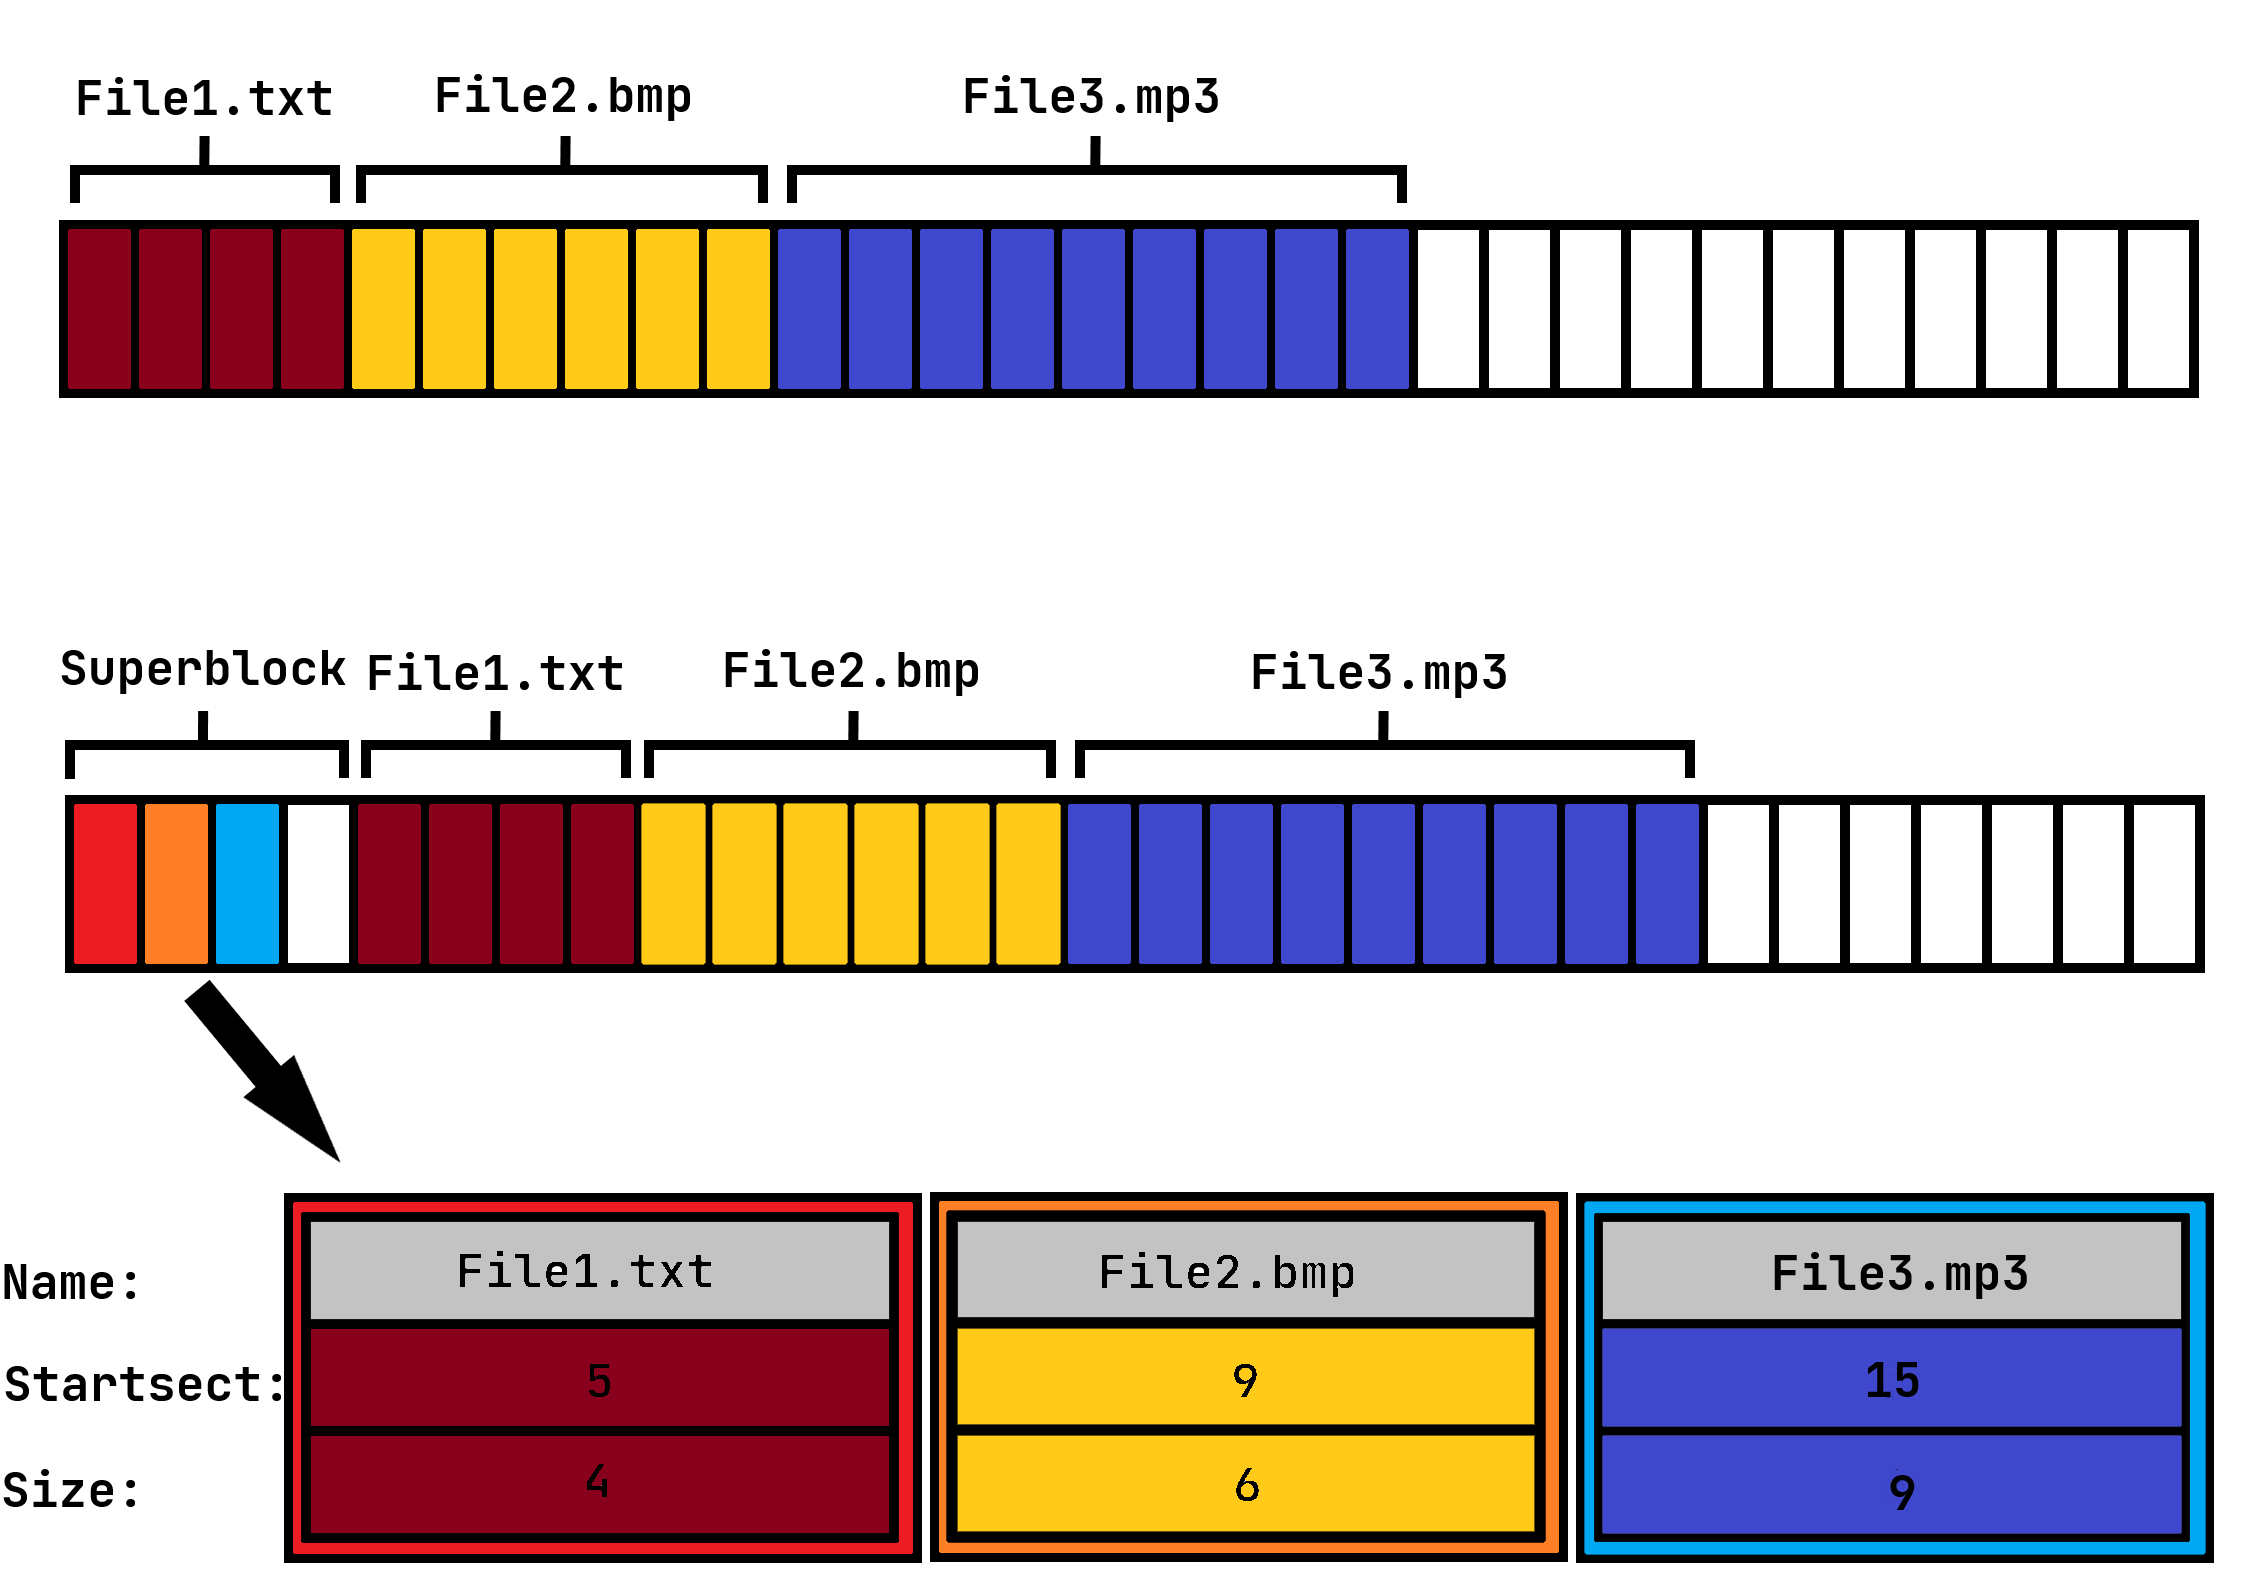
\includegraphics[width=350px]{filesystems.png}
	\centering
\end{figure}

The FS supports now various files and
because it works so well we start to organize our files. Organizing files requires \textit{directory}
support for Directories, also known as \textit{folders} on Windows, are filesystem objects that
\textit{"contain"} other files or. We decide to treat directories as regular files, except that we
add a flag in the inode that marks it as a directory. In these directory entry files, i.e. the actual
content of the directory, we can store the inode number of files and directories that are \textit{"stored"}
in it. Our hierarchical filesystem is built like a tree turned upside down, there is the root and every
subdirectory is a branch (directory) or a leaf (regular file). Now that files are organized, there is need
for a way to access them accordingly.

The next step is adding mechanisms for \textit{path traversal} i.e. the
ability to specify the position of a file that is nested within multiple directories. This is done by
checking all the inodes in the directory until a file name matching an inodes file name field is
found. If the path traverses multiple directories, the previous step of looking for inodes with a
matching file name is done recursively.


\textit{Note: For readers used to Windows, the path separator \texttt{/} is a \texttt{\textbackslash}}
Note that storing the file name in the inode itself can be a
bad idea because an inode is of fixed size and file name sizes vary greatly. One either has to preallocate a large inode size for a long filename
or force short file names to safe storage space. This is very restrictive but there is a solution.
Instead of storing the file name in the inode, it can be stored \texttt{"inside"} the parent directory,
together with the inode number. This means that the contents of a directory entry file would look similar 
to this:

\begin{figure}[h]
	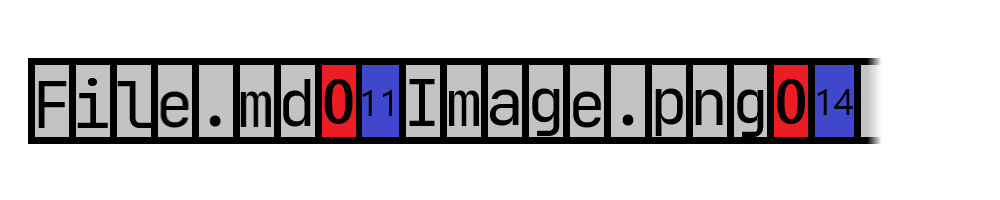
\includegraphics[width=350px]{disklayout.png}
	\caption{Layout of an example directory entry file \textit{"containing"} \texttt{File.md} and \texttt{Image.png}}
	\centering
\end{figure}

Every character in a box represents a byte on the disk. Notice the \texttt{\textbackslash 0} in the red field,
it is our file name string terminator and tells us that the following byte in blue is to be interpreted
as an inode number. After the inode number, the name of the next file starts and it is terminated with the next \texttt{\textbackslash 0}, which is again
followed by the inode number of the file. If the byte after an inode number is a \texttt{\textbackslash 0} the FS knows
that the directory doesn't have any more files.

Let us recap what we have looked at so far.
We have the superblock that contains metadata about files in per-file inodes. The inode stores the
location of a file on the disk and contains a field that describes whether it is a regular file or a
directory. The directory contains the file names and the inode numbers of the files and subdirectories
that are inside the directory. A file path (such as \texttt{pictures/summer21/img012.png}) can
be used to find the inode of the corresponding file and then the file location on the storage medium.

Our FS is very advanced now. Nonetheless, some things must be cleared up first. Because the name of
a directory is stored within its \textit{parent directory} (the directory that contains the subdirectory)
there must be a directory that does not have a name, because it does not have a parent directory
(unless there are infinitely many directories or a circular filesystem). This directory is the \textit{root
directory} and every other directory is either a direct or indirect subdirectory. The root directory
is often shown as a plain \texttt{/}. Windows users can think of it as the \texttt{C:\textbackslash} drive but that is actually not
entirely the case. We will explain why shortly, but there are some things that are important to know
first. If a path starts with the \texttt{/} such as \texttt{/home/Terry/tasks.txt} then the path is an \textit{absolute
path}. There is also a relative path and it depends on the \textit{current working directory}. Let's say that
a program is run from \texttt{/home/Terry/}. The current working directory is the aforementioned one. If the 
program wants to read the file \texttt{homework.txt} it can use the relative path to specify the file it
wants to read. The full path of the file is actually “/home/Terry/homework.txt“ but because the OS
knows the current working directory (\textit{cwd}) it can resolve the inode number of the file. Relative paths
are very convenient but they still lack a feature in our FS. If we want to specify a path of the parent
directory that does not traverse the \textit{cwd}, we must give the absolute path of the parent directory and
then the following subdirectories. But this is another issue that can be solved. Every directory
contains at least 2 entries (with the exception of the root directory). These are \texttt{.} and \texttt{..}. The
\texttt{.} is a directory entry file that points to itself. An example to understand it better is lets say
directory \texttt{/home/Terry/pics} has the inode number 8 and its parent directory has the inode number 6.
The directory entry file will contain the following:
\newline
\center
\begin{lstlisting}
'.' '\0' '\x08' '.' '.' '\0' '\x06' '\0'
\end{lstlisting}
\raggedright
The first entry in the directory \texttt{'.'} points to itself. This means that in a relative path a \texttt{'.'}
points to the directory itself. From a viewpoint in \texttt{/home/}, \texttt{'.'} is equal to \texttt{/home/}.
This is not very spectacular but if you look at the file directory above you can see that \texttt{'..'} points
to a file with inode 6. This is the parent directory of \texttt{'.'}. This is where it gets interesting. A
relative path can now contain a \texttt{'..'} and now we are able to give a relative path of every single file
on the filesystem. \texttt{../../} is the path of the parent's parent directory. Unlike the \texttt{'..'}, the \texttt{'.'}
does not have an effect on the path. \texttt{../pictures/pic.jpeg} is equal to \texttt{../pics/././tree.jpeg}.
With our fully fledged FS there are also some speed improvements. If we would like to move a 
file from \texttt{pics/} to the parent directory the FS only has to delete the entry of the <file to be moved> 
from the \texttt{pics/} directory entry file and write the file name and inode number into the directory 
entry file of \texttt{'..'}. This is a lot faster than copying the contents of the <file to be moved> and
writing them to a new file and deleting the old file. This FS also allows the renaming of open 
files, something that Windows still cannot do reliably. Windows simply queues the name change and commit 
it only after the file has been closed.

\subsection{Journaling filesystems}

Readers that have worked on old machines with primitive filesystems may have encountered one of the
most annoying things when trying to get work done: A crash. Back in the days a crash could mean that
the subsequent reboot of the system took hours to complete. This is because the system crashed while
something was being written to disk and resulted in filesystem corruption because of an unfinished
write operation to the storage medium. Usually this was just an issue when a write access to the
superblock or other filesystem specific data structures was unexpectedly interrupted. In that case a
time consuming disk recovery had to be run to find and fix the error. Journaling file systems came to
fix the issue. A new area on the disk got assigned to the \textit{journal file}. Whenever a write operation
to the disk is queued the FS writes the write parameters to the journal. This includes the sectors
that should be written to and the length of the data to be written to the storage medium. After the
write operation has been completed successfully the FS clears the journal by overwriting it. Whenever
the system boots up the OS, the filesystem checks the journal and if it finds an
unfinished query listed in the journal it will just fix the query. There is no need to check the
entirety of the FS and if the journal is empty, the OS can just continue starting up normally.
The journal file is not really a file but rather just a few sectors at a fixed location totaling a
fixed size for faster access times. Regular files might move around on the disk if they grow in size
or some other cases. In summary, a modern filesystem consists of the superblock storing all
filesystem objects metadata in inodes, a data structure that keeps track of (un)used sectors, a journal and
finally a vast, organized area that holds the contents of regular files and all directory entries.
